\subsubsection{VDBMS Architecture}
\label{sec:impl}


%-haskell
%-any dbms
%-manually generate vdb explained in expr
%-provide v-sch
%-input: vdb, vsch(==> valid configs), vq
%-arch fig
%-explain arch
%\point{impl in haskell on top of any dbms using haskell's type class.}
%To interact with VDBs using v-queries, we implement 
%\emph{Variational Database Management System (VDBMS)}.
%VDBMS is implemented in Haskell. VDBMS sit on 
%top of any DBMS that the user desires and used to store their data 
%%\arashComment{I did not find any explanation on how v-tables are stored in an RDBMS.} 
%%\resp{it is exactly implemented as formalized in v-table section.}
%%\responded
%in form of v-tables, explained in \secref{vtab}.
%%To acquire an extensible system we implement 
%To support running VDBMS with multiple different plain relational DBMS backends,
%we provide
%a shared interface
%for connecting to and inquiring information from a DBMS and
%instantiate it for different database engines such as PostgreSQL and
%MySQL. 
%%\rewrite{any dbms that has a library in haskell that has a function
%%that returns the result to the user. eg that doesn't satisfy this is 
%%database.sqlite3. } --> The following addresses this:
%An expert can extend VDBMS to another database engine by
%writing methods for connecting to and querying from the database.

%\input{sections/implVar}
%\point{vdb and vschema and config (bottom of fig).}
\section{VDBMS Architecture}
\label{sec:arch}

\figref{arch} shows the architecture of VDBMS.
% and its modules.
%For now, 
We assume a VDB and its variational schema are generated by an 
expert and are stored in a DBMS.
%, we return to generation of VDBs in 
%\secref{exp-disc}. 
A VDB can be \emph{configured} to its plain relational 
database variants
%, if desired by a user, 
by providing the configuration
of the desired variant, \figref{vdb-conf}.
For example, a SPL developer configures a VDB to produce 
software and its database for a client.
%To configure a VDB, VDBMS requires a list of valid configurations.
%Remember that the feature model is a feature expression that 
%encodes all valid configurations. Hence, solving the feature model
%by a SAT solver results in the list of valid configurations.


\begin{figure}
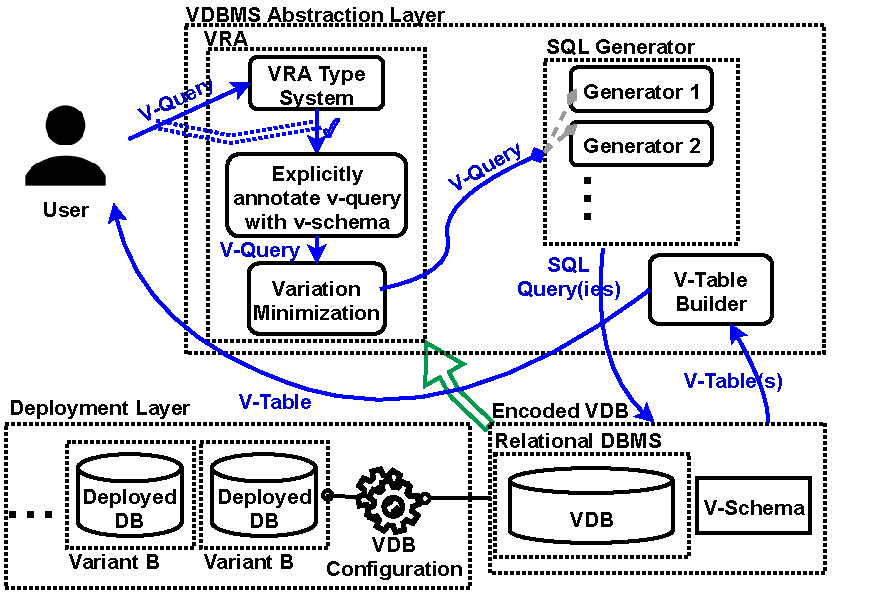
\includegraphics[width = \linewidth] {figs/arch/arch8.pdf}
\caption[VDBMS architecture and execution flow of a variational query]{VDBMS architecture and execution flow of a variational query. 
The dotted double-line from the input variational query
% to explicitly annotate variational query module
indicates the dependency of passing the variational query to this module
only if it is valid. 
The dashed gray arrows with diamond heads demonstrate
an option for the flow of the variational query. 
%We examine taking different routes
%to evaluate a variational query, resulting in various approaches in \secref{apps}.
The blue filled arrows track the data flow, the green hollow arrows 
indicate an input to a module.}
\label{fig:arch}
\end{figure}


%\point{flow of vq in vdbms.}
%Given a VDB and its variational schema, 
To extract information from a VDB, 
a user inputs a variational query \vQ\ to VDBMS.
%
First, \vQ\ is checked by the \emph{type system}.
%, explained in 
%First, \vQ\ is type-checked by the VRA type system introduced in 
%\secref{type-sys}. 
If the query is ill-typed, the user gets an error explaining what part of the 
query violated the variational schema.
%, shown in \exref{q-violate-sch}.
%\moredet{maybe give an ex of an error user will see! ref to ex of error given
%in \secref{type-sys}}
Otherwise, 
\vQ\ is explicitly annotated by the schema and
%defined in \secref{constrain},
%to ensure variation-preserving property w.r.t. variational schema throughout the execution flow of variational query 
%in the system and then
%
%Then, it 
is passed to the \emph{variation minimization} module,
% introduced in 
%\secref{var-min}, 
to simplify \vQ.
%minimize the variation of \vQ\ and apply
%relational algebra optimization rules. 
%
The simplified query is then sent to the \emph{generator} module where
SQL queries are generated from variational queries by different approaches explained 
in \secref{apps}.
%, \secref{apps} provides three
%approaches for this.
%\TODO{
%\exref{q-flow} in \appref{sql-gen} demonstrates the flow of a variational query through
%VDBMS.}
%\wrrite{have examples for each approaches. of mainly the final sql}

\begin{comment}
To generate runnable queries w.r.t. the underlying DBMS,
the minimized query \ensuremath {\VVal \vQ} is passed to 
the \emph{translate to RA} module that could use either 
configuring or grouping of variational queries, explained in \secref{vra-sem},
to generate RA queries. The generated 
queries are then sent to the \emph{SQL generator} module which generates
SQL queries in various ways from the relational algebra queries, explained
in \secref{sql-gen}.
%\moredet{in app have an ex of all this happening!}
\end{comment}

%\point{vtab builder.}
%Having generated a/multiple SQL query/ies, it/they is/are now run over the underlying 
%VDB.
All generated SQL queries are then executed on the underlying VDB.
% (stored in a DBMS desired by the user). 
 The result could be either 
a variational table or multiple variational tables, depending on the approach chosen by
%the translator to RA and 
the SQL generator. The variational table(s) is passed
to the \emph{variational table builder}
%\dropit{could drop \secref{vtab-build} and explain it here!}
%explained in \secref{vtab-build}, 
to create one variational table that filters out 
duplicate and invalid tuples, shrinks presence conditions, and 
eventually, returns the final variational table to the user.
Note that the variational table builder module uses the accumulation
functions introduced in \secref{accum} in addition to filtering out tuples and 
cleaning a variational table. 


%\input{sections/sqlGen}

